\section{Analysis and Results}
\label{sec:description_3}


In order to test our model we developed a Matlab simulation for the $2$-player version of the game and for the $3$-player version, the simulations are available in the Appendix \ref{ap:d}. When defining our game space $\Gamma$ in Section \ref{subsec:pirates_initialstate} we defined a number of variable parameters, such as: the entanglement coefitient $\gamma$; the coin distributions $\alpha_{ij}$; the strategies $\mathcal{U}_{j}$ that the players might use (restricting the operator space $\mathsf{SU}(2)$).

According to \cite{Du} when the entanglement is maximal, $\mathcal{U}(\pi, 0)$ is the optimal counter-strategy for $C$ (represented by the identity marix), $\mathcal{U}(0, \frac{\pi}{2})$ is the optimal counter strategy for $\mathcal{U}(\pi, 0)$, $D$ becomes the optimal counter-strategy for $\mathcal{U}(0, \frac{\pi}{2})$, and $C$ becomes an optimal counter strategy for $D$.

\subsection{$2$ Player Game}
\label{subsec:2playergame}

We simulated the Pirate Game for $2$-players according to the rules defined for our quantum model in Section . The simulation can be consulted for reference in Appendix \ref{ap:d}. The classical sub-game with $2$-players can be represented in Table \ref{tab:classico2jogadores_analise}. It is a strictly determined game, that means that there is at least a Nash Equilibrium when the players choose pure strategies\cite{Leyton-Brown2008:Essentials_Game_Theory}. In this case the outcome of the game is $(100, 0)$, when the players, use the strategies $C_{1}$ and $D_{2}$.  In the quantum game we can find the following $4$ pure quantum strategies :

\begin{itemize}

\item $I$

\item $D$

\item $\mathcal{U}( \pi, 0)$ - the quantum equivalent of a defection operator.

\item $\mathcal{U}( 0, \frac{\pi}{2})$ - the quantum equivalent of a cooperation operator.

\end{itemize}

The expected utility when players can choose only pure quantum strategies and the game is maximaly entangled is shown in Figures \ref{fig:pg_2players_99_0_1:1} and \ref{fig:pg_2players_99_0_1:2}. When each player has access to the $4$ quantum strategiesnthe game is still strictly determined with a Nash Equilibrium outcome $(100,0)$.

\begin{table}[h]
\begin{center}
\begin{centering}
\begin{tabular}{ccc}
\hline 
  & Player 2: C & Player 2: D\tabularnewline
\hline 
Player 1: C & (100, 0) & (100, 0)\tabularnewline
Player 1: D & (100, 0) & (-200, 100.5)\tabularnewline
\hline 
\end{tabular}

\par\end{centering}
\caption{Representation of the $2$ player sub-game in normal form.}
\label{tab:classico2jogadores_analise}
\end{center}
\end{table}

\begin{figure}[h!]
\centering 
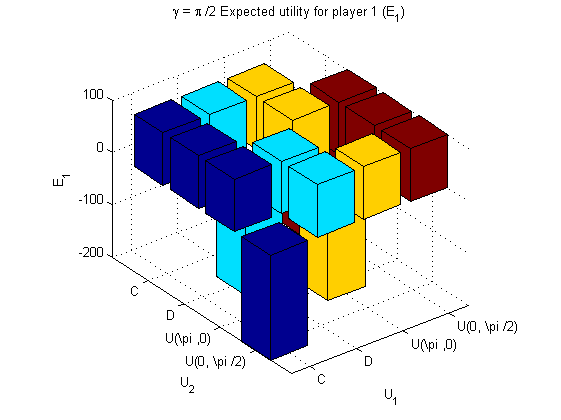
\includegraphics[scale=0.60]{Figures/1.5qubit/p2_E1.png}
\caption{Expected utility for player $1$, when both players have access to pure quantum strategies and the entanglement is maximum. }
\label{fig:pg_2players_99_0_1:1}
\end{figure}

\begin{figure}[h!]
\centering 
\includegraphics[scale=0.60]{Figures/1.5qubit/P2_E2.png}
\caption{Expected utility for player $2$, when both players have access to pure quantum strategies and the entanglement is maximum. }
\label{fig:pg_2players_99_0_1:2}
\end{figure}


\subsection{$3$ Player Game}
\label{subsec:3playergame}


\subsubsection{The captain proposes: $(99, 0, 1)$}
\label{subsubsec:3playergame99}

The move $(C_1,D_2,C_3,C_4,D_5)$ with a proposal of $(\alpha_{1}, \alpha_{2}, \alpha_{3}) =(99, 0, 1)$ represents Nash Equilibrium of the classic Pirate Game (for $3$ players). In the classical version, when the players chose at least $2$ operators $Cooperate$ on the initial proposal the game ends right away, and the first proposal, made by player $1$, is accepted ($Accepted 1$ or $A_{1}$). 

This game is a strictly determined game because it has a pure-strategy Nash Equilibrium.

After the players make their strategic moves and the disentangle operator $\mathcal{J}^{\dagger}$ is applied, and the payoff functionals are calculated given the final state. The final state will be calculated as shown in Equation \ref{eq:piratas_final_move_23}.

\begin{equation}
\vert\psi_{fin}\rangle=\otimes_{i=1}^{3}\otimes_{j\in\xi^{-1}(i)}\mathcal{U}_{j}\vert\psi_{ini}(\gamma)\rangle
\label{eq:piratas_final_move_23}
\end{equation} 

As expected from the problem definition when players use only classical strategies the entanglement coefficient will not affect the final expected utilities ($[ \mathcal{J} , C \otimes D \otimes C \otimes C \otimes D ] = 0 $).
An example of this behaviour is shown in Figure \ref{fig:pg_3players_99_0_1}, where we measure the probability $A_{1}$ (first proposal is accepted), $A_{2}$, and $R_{2}$, with different entanglement levels ($\gamma= \{ 0 , \frac{ \pi}{4}, \frac{\pi}{2} \} $).

\begin{figure}[h!]
\centering 
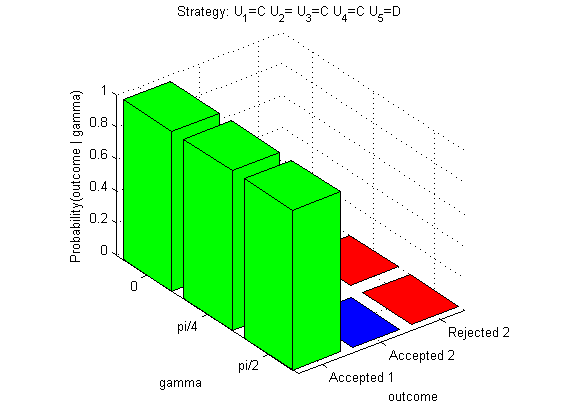
\includegraphics[scale=0.80]{Figures/1.5qubit/CDCCD.png}
\caption{When player play classical strategies the entanglement will not affect the final result. }
\label{fig:pg_3players_99_0_1}
\end{figure}

When each player chooses an operator from the set $O = \{ \mathcal{U} ( \theta , 0) , \theta \in (0, \pi) \}$ and $\gamma=0$ we have an equivalent to the classic mixed strategies. However for $\gamma >0$ the $\mathcal{U} ( \theta , 0)$ may present an interference behaviour that is inherently quantum. This effect is shown in Figures \ref{fig:pg_3players_99_0_1:2} and \ref{fig:pg_3players_99_0_1:2}, allowing us to understand the difference between the Bit-flip operator $D$ and $\mathcal{U} ( \pi , 0)$.



\begin{figure}[!h]
\centering 
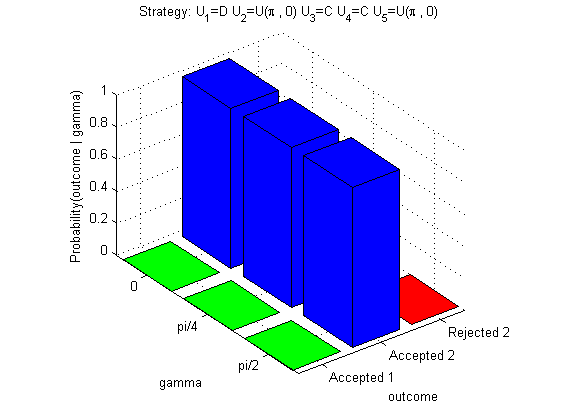
\includegraphics[scale=0.80]{Figures/1.5qubit/DUpi0CCUpi0.png}
\caption{Players use the operators . }
\label{fig:pg_3players_99_0_1:2}
\end{figure}

\begin{figure}[h!]
\centering 
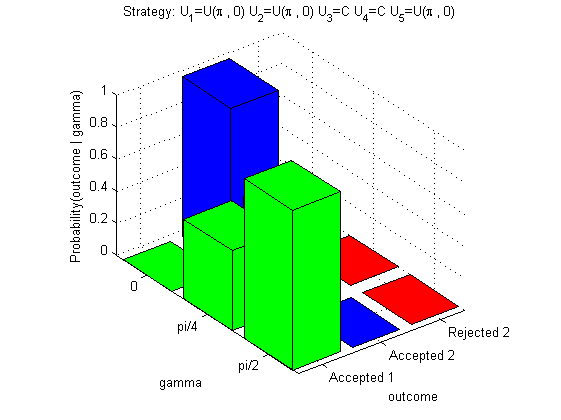
\includegraphics[scale=0.80]{Figures/1.5qubit/Upi0Upi0CCUpi0.png}
\caption{Unlike with the Bit-flip operator $D$, $\mathcal{U} (\pi, 0)$ is affected by the entanglement coefficient $\gamma$ in this case. }
\label{fig:pg_3players_99_0_1:3}
\end{figure}














\clearpage
\subsubsection{The captain proposes: $(100, 0, 0)$}
\label{subsubsec:3playergame100}

Suppose captain is greedy and proposes to get the 100 coins. In the classical Pirate Game this would pose a conflict with his self-preserving needs. 
A pertinent question would be if this Quantum Model of the Pirate Game would allow the first captain to approve that allocation proposal. 

If the captain is the only one with access to quantum strategies, and the other players do not know it and play the classical strategies $C$ (identity matrix) and $D$ (Bit-flip operator), there is a dominant quantum strategy that allows her to pass her proposal and get all the $100$ coins, for $\gamma = \frac{\pi}{2}$. Figure \ref{fig:pg_3players_99_0_1:4} provides an example that corroborates where we verify that player $1$ has a set of dominant strategies (for $\tau_{1} = \mathcal{U}_{1}(\pi,\phi), \phi \in (0, \frac{\pi}{2})$ or $\tau_{1} = \mathcal{U}_{1}(\theta,\frac{\pi}{2}), \theta \in (0, \pi)$). We verified experimentally that the sub-games with $2$ players (when $(C_{4},C_{5}), (C_{4},D_{5}), (D_{4},C_{5}), (D_{4},D_{5})$), did not affect this dominant strategy. If fact if we analyse the expected utility function for player $1$ ($E_{1}.$), and the Figure \ref{fig:pg_architecturegametree:extensiveform} representing the extensive form game, we verify that the the first captain is indifferent to the results of the sub-game with $2$-players, when both player play a classical strategy, because she is already dead. 

\begin{figure}[h!]
\centering 
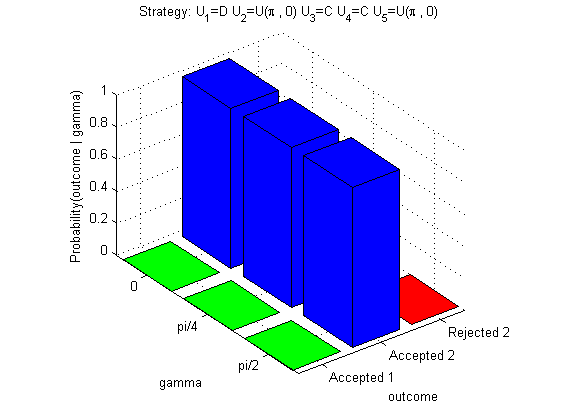
\includegraphics[scale=0.80]{Figures/1.5qubit/DUpi0CCUpi0.png}
\caption{Player $1$ uses the classical operator D. The probabilities don't change with the entanglement.  }
\label{fig:pg_3players_99_0_1:2}
\end{figure}

\begin{figure}[h!]
\centering 
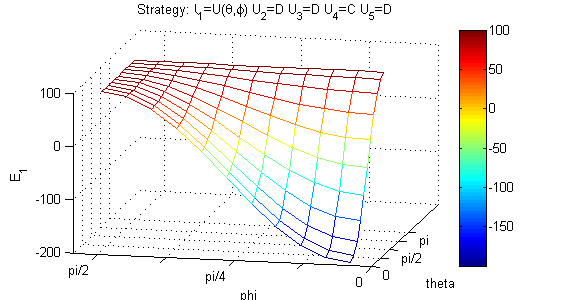
\includegraphics[scale=0.80]{Figures/1.5qubit/meanpirate.png}
\caption{Expected utility for player $1$ when she adopts a strategic move of the form $U_{1}(\theta,\phi)$ and the other players play $D_{2},D_{3},C_{4},D_{5}$. }
\label{fig:pg_3players_99_0_1:4}
\end{figure}

If players $2$ and $3$ know that the captain has access to quantum strategies, with a maximaly entangled game, and they have the restricted sub-set of pure classical strategies $C_{j}$ and $D_{j}$, if they both play $C$, the dominant strategy for the captain becomes $\tau_{1} = \mathcal{U}_{1}(0,0)$. Their best response becomes playing a mixed strategy where half the time they will play $C$ and the other half $D$. The best response for player $1$ in this case is to play a mixed quantum strategy where half the time she plays $\mathcal{U}(0,0)$, half $\mathcal{U}(0,pi/2)$.



\begin{figure}[h!]
\centering 
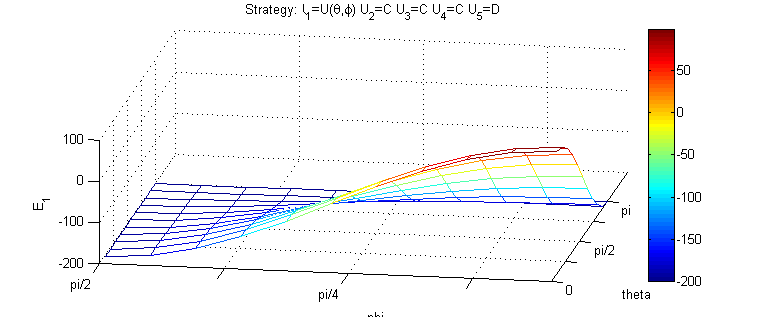
\includegraphics[scale=0.80]{Figures/1.5qubit/meanpirategetscrewed.png}
\caption{Players $2$ and $3$ use a mixed classical strategy to choose the operators $O_{2}$ and $O_{3}$, where half the time they will play $C$ and the other half $D$. }
\label{fig:pg_3players_99_0_1:2}
\end{figure}

\begin{figure}[h!]
\centering 
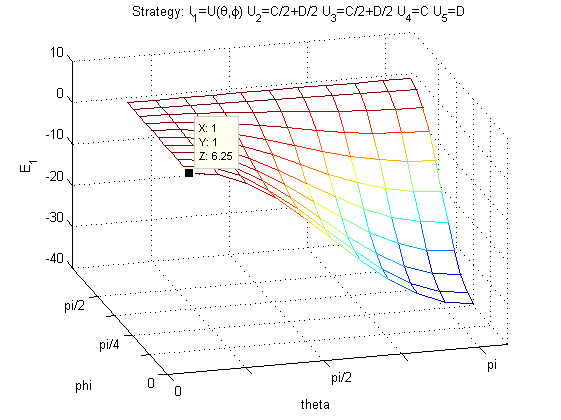
\includegraphics[scale=0.80]{Figures/1.5qubit/mixedclassical.png}
\caption{Players $2$ and $3$ use the operators $C_{2}$ and $C_{3}$. }
\label{fig:pg_3players_99_0_1:2}
\end{figure}

\begin{figure}[h!]
\centering 
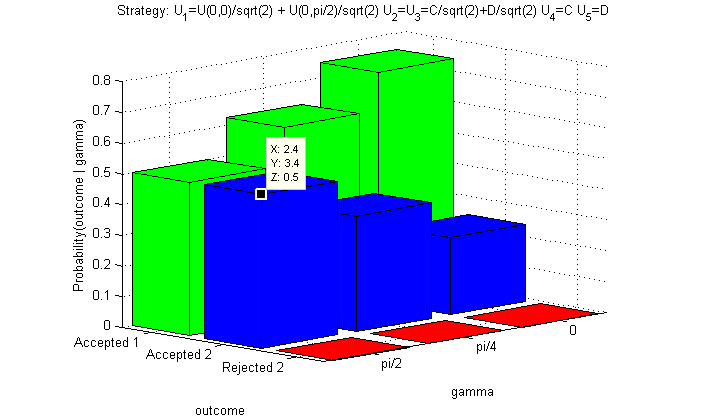
\includegraphics[scale=0.80]{Figures/1.5qubit/mixedmixedclassical.png}
\caption{Players $2$ and $3$ use the operators $C_{2}$ and $C_{3}$. }
\label{fig:pg_3players_99_0_1:2}
\end{figure}




\begin{comment}


The player $1$, the captain, needs two votes to pass her proposal. In order to answer our question we must analyse the expected utilities for all players where the initial proposal is accepted. Moreover we need to analyse an instance where the proposal is refused, when the players select the actions $(C,D,D)$. In the previous analysis we observed that player $2$ has a strong motivation to Defect in the first round, because in the second round she can pass the proposal with her vote alone, this means if the player $1$ wants to pass is proposal she should choose the $C$ operator.

 Our final state will be calculated as shown in Equation \ref{eq:piratas_final_move2_99anal}.



In Table \ref{tab:3playerDCC100} we notice that player $3$ will get a expected payoff of $0.5$ if she chooses to Defect.
\begin{table}[h]
\begin{center}
\begin{tabular}{cc}
  \putindeepbox[7pt]{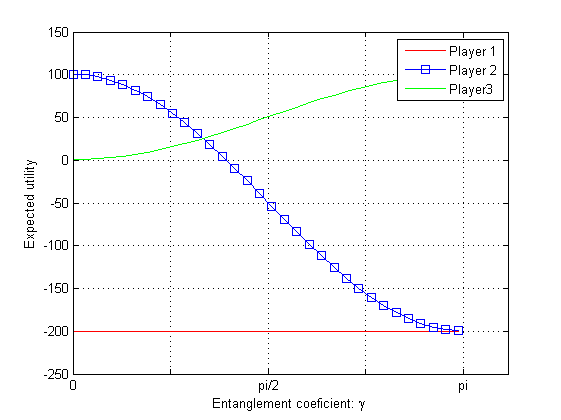
\includegraphics[scale=0.72]{3Accepted100/CDD_CC.PNG}}
\end{tabular}
\caption{Expected utility for $3$ players, where the players will use the $(Cooperate, Defect, Defect)$ operators in the first stage. In the second stage we represented the sub-game equilibrium of the game.  }
\label{tab:3playerDCC100}
\end{center}
 \end{table}


In Tables \ref{tab:3playerCDC100} and \ref{tab:3playerCCD100}, the expected utility function for player $3$ starts of as $0$ for $\gamma=0$ (which corresponds to the classical problem). The function presents a maximum when the system is maximally entangled; this maximum is $0.5$. If the proposal is accepted when the entanglement coefficient is $\gamma=\frac{\pi}{2}$ player $1$ will get a negative expected payoff (which means he will die under that condition).

\begin{table}[h]
\begin{center}
\begin{tabular}{c}
  \putindeepbox[7pt]{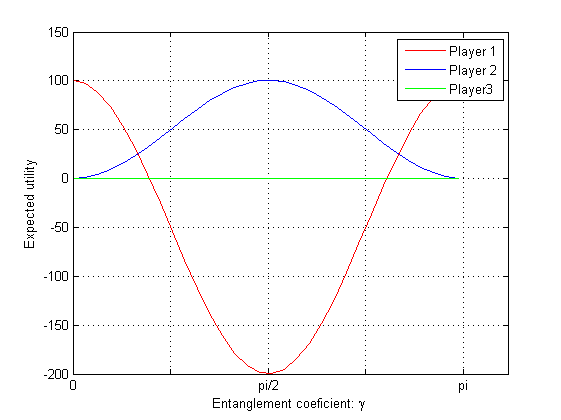
\includegraphics[scale=0.72]{3Accepted100/CCD.PNG}}
\end{tabular}
\caption{Expected utility for $3$ players, where the players will use the $(Cooperate, Cooperate, Defect)$ operators. }
\label{tab:3playerCCD100}
\end{center}
 \end{table}

\begin{table}[h]
\begin{center}
\begin{tabular}{c}
  \putindeepbox[7pt]{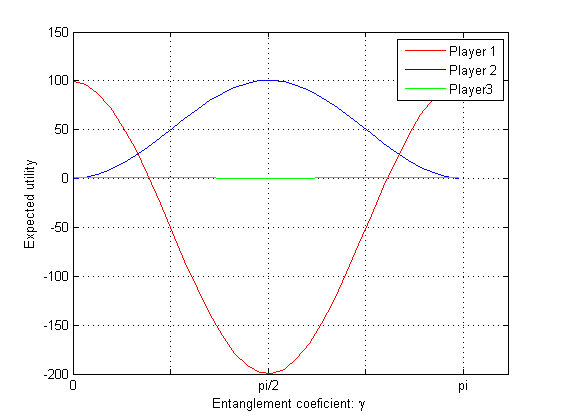
\includegraphics[scale=0.72]{3Accepted100/CDC.PNG}}
   
\end{tabular}
\caption{Expected utility for $3$ players, where the players will use the $(Cooperate, Defect, Cooperate)$ operators.}
\label{tab:3playerCDC100}
\end{center}
 \end{table}

The Table \ref{tab:3playerCCC100} presents an outcome where all the players vote in favour of the proposal. The players $2$ and $3$ have and expected utility of $0$, regardless the role of entanglement in the system.



\begin{table}[h]
\begin{center}
\begin{tabular}{c}
  \putindeepbox[7pt]{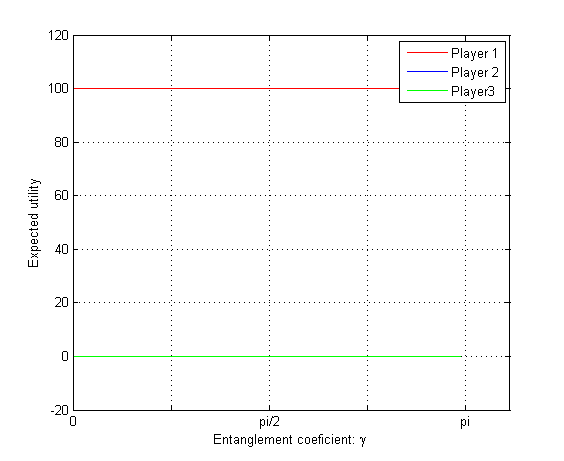
\includegraphics[scale=0.72]{3Accepted100/CCC.PNG}}
\end{tabular}
\caption{Expected utility for $3$ players, where the players will use the $(Cooperate, Cooperate, Cooperate)$ operators. The initial proposal is $(\alpha_{1}, \alpha_{2}, \alpha_{3}) =(100, 0, 0)$. }
\label{tab:3playerCCC100}
\end{center}
 \end{table}

From this simulation we can conclude that if the captain wants to pass her proposal for $\gamma=\frac{\pi}{2}$ there are $3$ equilibria when the player select the operators $(CDC)$, $(C,C,D)$, and $((C,D,D),(C,C))$. $(CDC)$, $(C,C,D)$ correspond to an accepted proposal. However player $1$ will get a negative payoff in any of this equilibria. 

We can interpret this in the context of the problem with the captain getting the coins as she proposed, but being immediately betrayed and killed by her fellow pirates who conspired in order for player $2$ to get all the coins, and player $3$ to become second in command.

Otherwise there is one Nash Equilibrium when the players select $((C,D,D),(C,C))$. Even in a quantum version, the captain needs to bribe player $3$ in order to approve her proposal and get a maximum of $99$ gold coins.


\end{comment}




